\documentclass{jlreq}

\usepackage{bm}
\usepackage{fancyhdr}
\usepackage{float}
\usepackage{graphicx}
\usepackage{listings}
\usepackage{xcolor}
\usepackage{caption}

\pagestyle{fancy}
\fancyhf{}
\fancyhead[R]{\thepage}

\renewcommand\thesubsection{(\alph{subsection})}

\title{言語処理プログラミング 課題4}
\author{22122502 川口 栄宗}
\date{提出日: \today}

\begin{document}

\maketitle
\clearpage

\section{作成したプログラムの設計情報}

\subsection{全体構成}

全体構成を図\ref{fig:module_graph}に示す.
\begin{figure}[H]
  \centering
  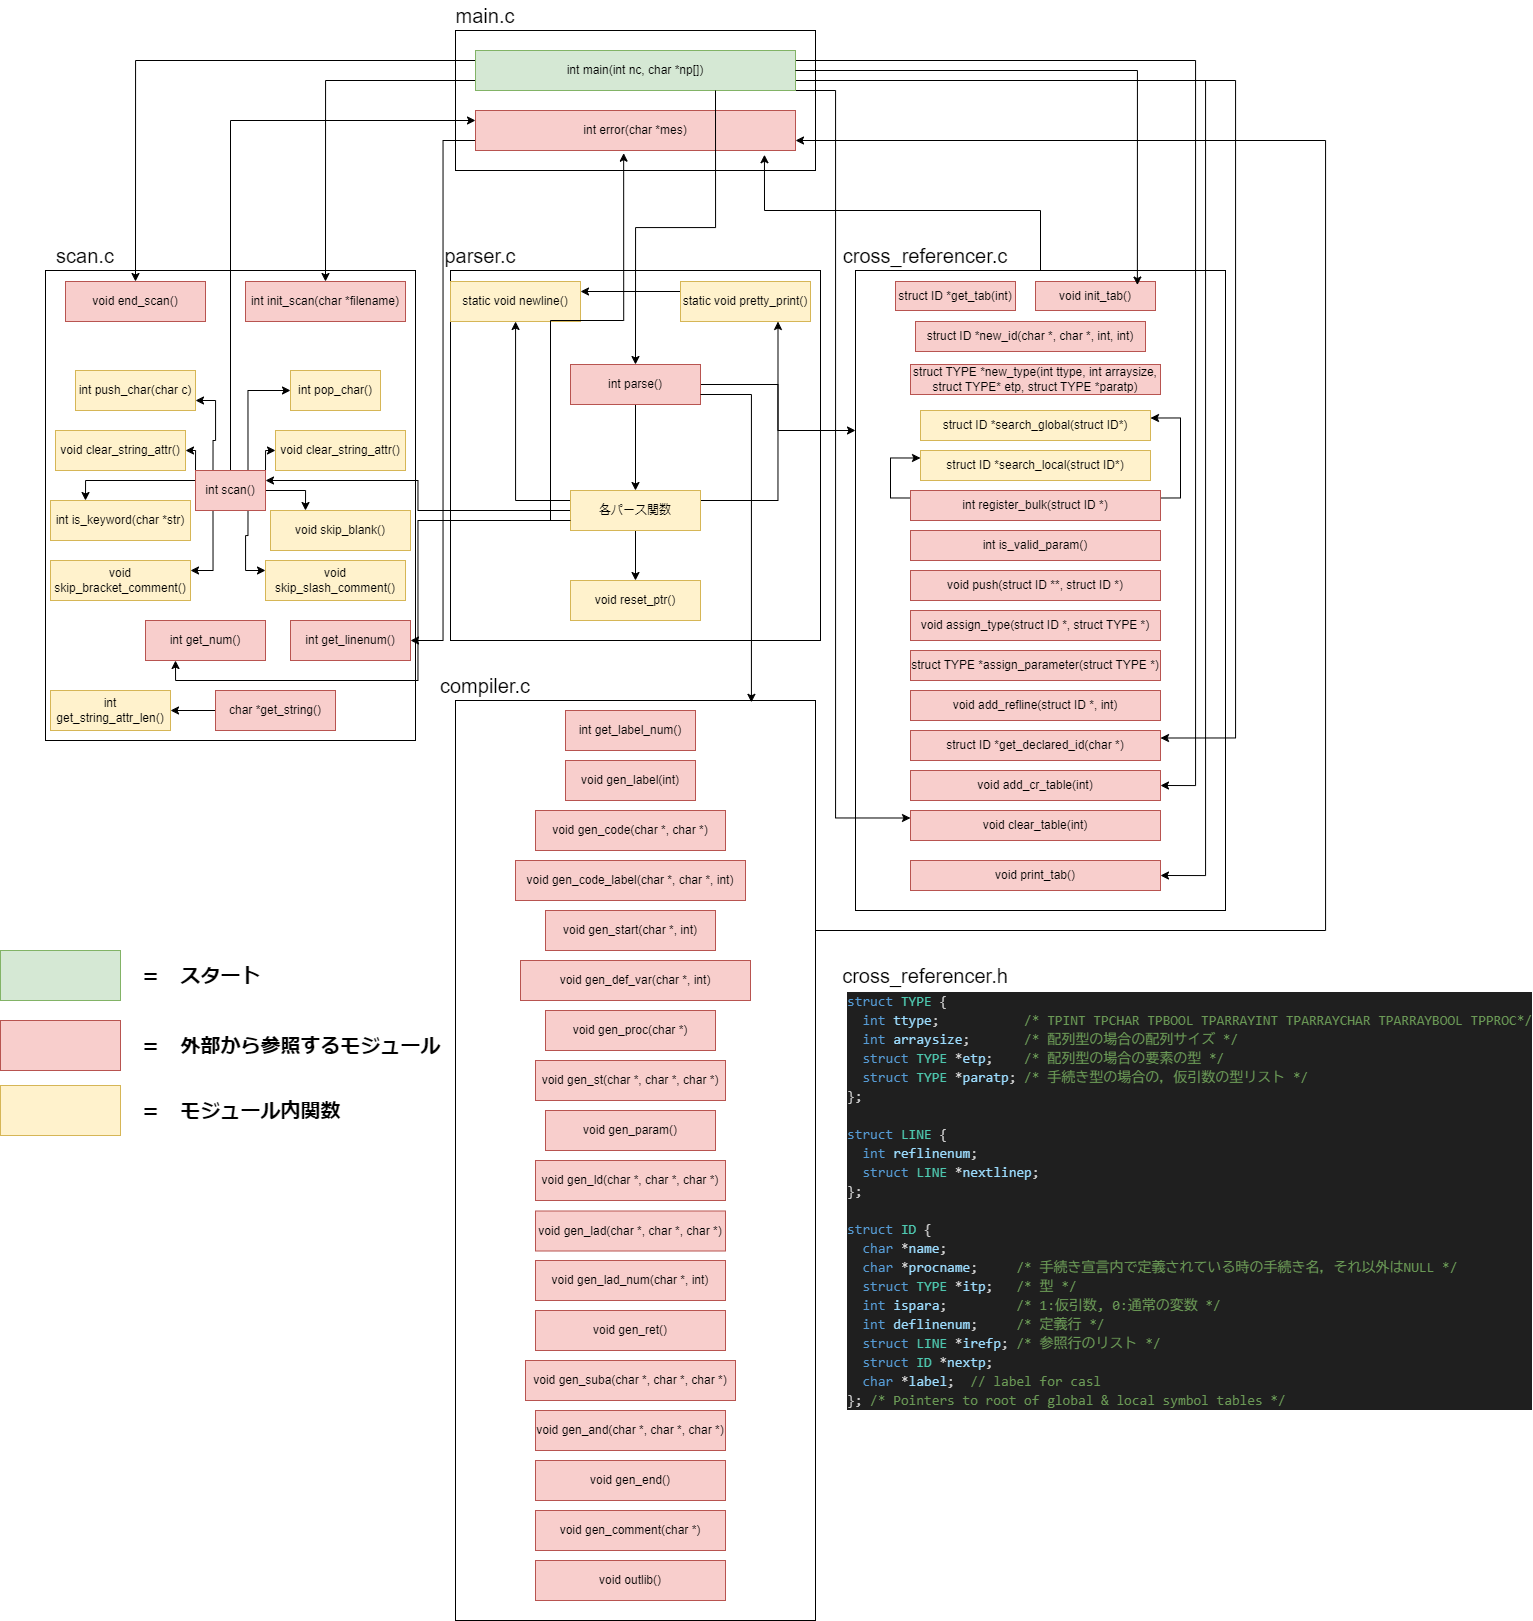
\includegraphics[width=\textwidth]{assets/lpp04_module.png}
  \caption{課題4のモジュール構成図}
  \label{fig:module_graph}
\end{figure}

\subsection{各モジュールごとの構成}

\subsubsection{main.c}
変数やモジュール機能は課題1~3からほぼ変更を加えていない.課題4で追加した機能として,
コマンドライン引数で与えられたファイル名をcsl形式に変換してカレントディレクトリを出力する機能,
cslファイルの開閉の部分を追加した.

\subsubsection{scan.c}
課題1~3で記載済み

\subsubsection{parser.c}
課題2で実装した構文解析を行い,制約についても解析を行う.
また,構文解析しながらクロスリファレンサのモジュールを呼び出して表を作成する.
表\ref{tab:parser_design}に課題4で追加した各変数とその意味について触れる.

\begin{table}[H]
  \centering
  \caption{parser.cの各変数とその意味}
  \begin{tabular}{|l|p{10cm}|}
    \hline
    変数         & 意味                                                       \\ \hline
    break\_label & break文などでループを抜ける時のラベル先を記憶する変数      \\
    var\_flag    & 変数を解析した場合に1になるフラグ                          \\
    left\_flag   & 左辺値とする場合に1にするフラグ                            \\
    addr\_flag   & コード生成の際に,計算結果がアドレスだった場合に立つフラグ \\ \hline
  \end{tabular}
  \label{tab:parser_design}
\end{table}

\subsubsection{cross\_referencer.c}
課題4で追加した部分として,既存の関数内にコード生成の実装を含めたり,構造体IDに変数のラベルを持つフィールドを追加した.
構造体の内容は図\ref{fig:module_graph}にて確認できる.
大域変数などは課題3に記載済みである.

\subsection{各関数の外部仕様}

\subsubsection{scan.c}
scan.cの関数の外部仕様を表\ref{tab:scan_func}に示す.

\begin{table}[H]
  \centering
  \caption{scan.cの関数の外部仕様}
  \begin{tabular}{|l|p{6cm}|l|p{3cm}|}
    \hline
    関数名                 & 機能              \\ \hline
    init\_scan             & 課題1から変更なし \\
    end\_scan              & 課題1から変更なし \\
    scan                   & 課題1から変更なし \\
    push\_char             & 課題1から変更なし \\
    pop\_char              & 課題1から変更なし \\
    clear\_string\_attr    & 課題1から変更なし \\
    is\_keyword            & 課題1から変更なし \\
    skip\_blank            & 課題1から変更なし \\
    skip\_bracket\_comment & 課題1から変更なし \\
    skip\_slash\_comment   & 課題1から変更なし \\
    get\_string\_attr\_len & 課題3から変更なし \\
    get\_linenum           & 課題3から変更なし \\
    get\_string            & 課題3から変更なし \\
    get\_num               & 課題3から変更なし \\ \hline
  \end{tabular}
  \label{tab:scan_func}
\end{table}

\subsubsection{parser.c}
parser.cの関数の外部仕様を表\ref{tab:parser_func}に示す.なお,課題3までで記載済みの分は省略し,課題4で追加した機能について触れる.

\begin{table}[H]
  \centering
  \caption{parser.cの関数の外部仕様}
  \scalebox{0.5}{
    \begin{tabular}{|l|p{15cm}|l|p{6cm}|}
      \hline
      関数名                          & 機能                                                                                                                                                                                                                                                           & 引数 & 戻り値                             \\ \hline
      parse\_program                  & プログラムの解析と同時に,START命令やCALL FLUSHのコード,RET,ライブラリコードの生成を行う.                                                                                                                                                                   & ~    & ~                                  \\
      parse\_block                    & ブロック解析を行う.副プログラム宣言を解析したときは,procnameをNULLにし,local\_tabをクロスリファレンス表に追加して元を削除する.また,reset\_ptr関数で諸々のポインタをNULLにリセットする.                                                                   & なし & 成功は0,エラーは-1                \\
      parse\_variable\_declaration    & 変数宣言部の解析を行う.変数の並びと型の情報をそれぞれ取得し,クロスリファレンサ用のテーブルに登録する.                                                                                                                                                       & なし & 成功は0,エラーは-1                \\
      parse\_variable\_names          & 変数名の並びを解析する.1つ1つの変数をテーブルに追加していく.                                                                                                                                                                                                 & なし & 成功は0,エラーは-1                \\
      parse\_variable\_name           & 変数名を解析する.変数名の文字列を大域変数nameに割り当て,行番号も大域変数deflinenumに割り当てる.                                                                                                                                                             & なし & 成功は0,エラーは-1                \\
      parse\_type                     & 型を解析し,型情報を作成して大域変数tpに割り当てる.                                                                                                                                                                                                           & なし & 成功は0,エラーは-1                \\
      parse\_standard\_type           & 標準型を解析する.array\_flagによって,配列の型なのか,普通の標準型なのかを場合分けし,得られた結果を戻り値として返す.                                                                                                                                        & なし & 成功は型番号,エラーは-1           \\
      parse\_array\_type              & 配列型を解析する.array\_flagを1にした上で解析を行い,parse\_standard\_type関数でどの配列の型なのかを取得し,戻り値として返す.                                                                                                                                & なし & 成功は配列の型番号,エラーは-1     \\
      parse\_subprogram\_declaration  & 副プログラム宣言を解析する.ttypeをTPROCとし,procidとproctpを用いて手続きに関する情報のテーブルへの追加と型情報の割り当てを行う.                                                                                                                             & なし & 成功は0,エラーは-1                \\
      parse\_procedure\_name          & 手続き名を解析する.手続き名の文字列をnameに割り当て,定義行をdeflinenumに割り当てる.                                                                                                                                                                         & なし & 成功は0,エラーは-1                \\
      parse\_formal\_parameters       & 仮引数を解析する.formal\_arg\_flagを1にし,変数の並びと型情報を取得してidをlocal\_tabに追加する.解析が終わったらformal\_arg\_flagを0に戻す.                                                                                                                 & なし & 成功は0,エラーは-1                \\
      parse\_compound\_statement      & 課題2から変更なし                                                                                                                                                                                                                                              & ~    & ~                                  \\
      parse\_statement                & 課題2から変更なし                                                                                                                                                                                                                                              & ~    & ~                                  \\
      parse\_condition\_statement     & 条件分岐を解析する.条件式の型がboolean型を満たしているかを確認している.                                                                                                                                                                                      & なし & 成功は0,エラーは-1                \\
      parse\_iteration\_statement     & 繰り返し文を解析する.繰り返しの条件式の型がboolean型を満たしているかを確認している.                                                                                                                                                                          & なし & 成功は0,エラーは-1                \\
      parse\_exit\_statement          & 課題2から変更なし                                                                                                                                                                                                                                              & ~    & ~                                  \\
      parse\_call\_statement          & 手続き呼び出し文を解析する.手続き名をprocname\_tmpが取得し,それをもとに既存のテーブルに検索をかけてポインタ変数varに渡す.既に定義されていたら参照行を追加し,未定義の場合はエラーとする.                                                                   & なし & 成功は0,エラーは-1                \\
      parse\_expressions              & 式の並びを解析する.手続きの仮引数に相当するため,手続きの情報をもつvarを基に正しく型が設定されているかを確認していく.                                                                                                                                        & なし & 成功は0,エラーは-1                \\
      parse\_return\_statement        & 課題2から変更なし                                                                                                                                                                                                                                              & ~    & ~                                  \\
      parse\_assignment\_statement    & 代入文の解析を行う.左辺部と式の型を比較して,型が等しいかつ標準型かどうかを判定する.また,型が違う場合でも適切な型であるか確認する.                                                                                                                         & なし & 成功は0,エラーは-1                \\
      parse\_left\_part               & 左辺部の解析を行う.変数を解析して得た型を戻り値として返す.                                                                                                                                                                                                   & なし & 成功は型番号,エラーは-1           \\
      parse\_variable                 & 変数の解析を行う.変数名の文字列でテーブルに検索をかけ,結果をvarに格納する.定義されている変数を参照した場合は,varに参照行を追加する.また,配列の要素であった場合は,添え字が符号なし整数であるかどうかを確認し,問題がなければ変数の型を戻り値として返す. & なし & 成功は型番号,エラーは-1           \\
      parse\_expression               & 式の解析を行う.単純式1つの場合はその型を,関係演算子で繋がれた場合は2つの型が同じかどうかを判定する.                                                                                                                                                         & なし & 成功は型番号,エラーは-1           \\
      parse\_simple\_expression       & 単純式を解析する.符号があればその後に符号なし整数が続くかどうかを判定し,単項1つである場合はその型を返し,和差の場合は2つの型が適切なものかどうかを判定してから型を返す.                                                                                     & なし & 成功は型番号,エラーは-1           \\
      parse\_term                     & 単項を解析する.因子1つであればその型を返し,積で繋がれた場合は2つの型が正しいか判定して結果を返す.                                                                                                                                                           & なし & 成功は型番号,エラーは-1           \\
      parse\_factor                   & 因子を解析する.条件分岐でどの因子かを選び,得られた型を返す.                                                                                                                                                                                                 & なし & 成功は型番号,エラーは-1           \\
      parse\_constant                 & 定数を解析する.符号なし整数か論理値かchar型かを判定して,その結果を返す.stringトークンの長さが1でない場合は定数として扱えないためエラーとする.                                                                                                              & なし & 成功は型番号,エラーは-1           \\
      parse\_multiplicative\_operator & 乗法演算子を解析する.字句が乗法演算子の種類を表しているため,それを戻り値として返す.                                                                                                                                                                         & なし & 成功は乗法演算子の字句,エラーは-1 \\
      parse\_additive\_operator       & 加法演算子を解析する.字句が加法演算子の種類を表しているため,それを戻り値として返す.                                                                                                                                                                         & なし & 成功は加法演算子の字句,エラーは-1 \\
      parse\_relational\_operator     & 関係演算子を解析する.字句が関係演算子の種類を表しているため,それを戻り値として返す.                                                                                                                                                                         & なし & 成功は関係演算子の字句,エラーは-1 \\
      parse\_input\_statement         & 入力文を解析する.括弧内の変数の型を取得し,符号なし整数かchar型かを判定している.                                                                                                                                                                             & なし & 成功は0,エラーは-1                \\
      parse\_output\_statement        & 課題2から変更なし                                                                                                                                                                                                                                              & ~    & ~                                  \\
      parse\_output\_format           & 出力指定を解析する.出力指定が式であったときに型を取得して,標準型であるかどうかを確認している.                                                                                                                                                               & なし & 成功は0,エラーは-1                \\
      parse\_empty\_statement         & 課題2から変更なし                                                                                                                                                                                                                                              & ~    & ~                                  \\ \hline
    \end{tabular}
  }
  \label{tab:parser_func}
\end{table}

\subsubsection{cross\_referencer.c}
cross\_referencer.cの関数の外部仕様を表\ref{tab:cross_referencer_func}に示す.

\begin{table}[H]
  \centering
  \caption{cross\_referencer.cの関数の外部仕様}
  \scalebox{0.7}{\begin{tabular}{|l|p{6cm}|p{7cm}|p{4cm}|}
      \hline
      関数名            & 機能                                                                                             & 引数                                   & 戻り値                        \\ \hline
      init\_tab         & 大域名用のテーブル,副プログラム宣言内用のテーブル,クロスリファレンス表のテーブルを初期化する. & なし                                   & なし                          \\
      new\_id           & 変数や手続き名のIDのインスタンスを作成する.                                                     & char *, char *, int, int               & struct ID *型のインスタンス   \\
      new\_type         & 型情報のインスタンスを作成する.                                                                 & int, int, struct TYPE *, struct TYPE * & struct TYPE *型のインスタンス \\
      search\_global    & 大域名用の記号表から指定したIDを検索する.                                                       & struct ID *                            & struct ID *                   \\
      search\_local     & 局所名用の記号表から指定したIDを検索する.                                                       & struct ID *                            & struct ID *                   \\
      register\_bulk    & 記号表をまとめてglobal\_tabかlocal\_tabに登録する.                                              & struct ID *                            & 成功は0,エラーは-1           \\
      is\_valid\_param  & local\_tabを探索して仮引数内の型が標準型かどうか確認する.                                       & なし                                   & 成功は0,エラーは-1           \\
      push              & 引数で与えられたheadにIDを追加する.                                                             & struct ID **, struct ID *              & なし                          \\
      assign\_type      & 引数で与えられた記号表に型情報を付与する.                                                       & struct ID *, struct TYPE *             & なし                          \\
      assign\_parameter & 引数で与えられた手続きの型情報に仮引数内の型情報を追加する.                                     & struct TYPE *                          & struct TYPE *                 \\
      add\_refline      & 引数で与えられた記号表に参照行を追加する.                                                       & struct ID *, int                       & なし                          \\
      get\_declared\_id & 引数で与えられた文字列からlocal\_tabとglobal\_tabを探索し,一致した記号表を返す.                & char *                                 & struct ID *                   \\
      add\_cr\_table    & 引数で指定した番号に応じて(0ならlocal\_tab,1ならglobal\_tab),クロスリファレンス表に追加する.  & int                                    & なし                          \\
      clear\_table      & 引数で指定した番号に応じて(0ならlocal\_tab,1ならglobal\_tab,2ならcr\_tab),表の削除を行う.    & int                                    & なし                          \\
      print\_tab        & クロスリファレンス表cr\_tabの内容を標準出力する.                                                & なし                                   & なし                          \\ \hline
    \end{tabular}}
  \label{tab:cross_referencer_func}
\end{table}


\section{テスト情報}
\subsection{テストデータ}
\subsubsection{ブラックボックステスト}
ブラックボックステストには用意されていたテストデータを用いた.テストデータを以下に示す.
\begin{itemize}
  \item sample11.mpl
  \item sample011.mpl
  \item sample11p.mpl
  \item sample11pp.mpl
  \item sample12.mpl
  \item sample012.mpl
  \item sample12cr.mpl
  \item sample12crlf.mpl
  \item sample012eof.mpl
  \item sample12lf.mpl
  \item sample12lfcr.mpl
  \item sample012n.mpl
  \item sample012neof.mpl
  \item sample012s.mpl
  \item sample012seof.mpl
  \item sample13.mpl
  \item sample013.mpl
  \item sample14.mpl
  \item sample014.mpl
  \item sample014a.mpl
  \item sample014b.mpl
  \item sample14p.mpl
  \item sample15.mpl
  \item sample15a.mpl
  \item sample16.mpl
  \item sample17.mpl
  \item sample18.mpl
  \item sample19p.mpl
  \item sample2a.mpl
  \item sample02a.mpl
  \item sample21.mpl
  \item sample021.mpl
  \item sample22.mpl
  \item sample022.mpl
  \item sample23.mpl
  \item sample023.mpl
  \item sample24.mpl
  \item sample024.mpl
  \item sample24a.mpl
  \item sample25.mpl
  \item sample025.mpl
  \item sample025a.mpl
  \item sample25t.mpl
  \item sample26.mpl
  \item sample026.mpl
  \item sample26a.mpl
  \item sample27.mpl
  \item sample28p.mpl
  \item sample29p.mpl
  \item sample31p.mpl
  \item sample032p.mpl
  \item sample33p.mpl
  \item sample34.mpl
  \item sample35.mpl
  \item sample41.mpl
\end{itemize}

\subsubsection{ホワイトボックステスト}
ブラックボックステストに用いたデータと同じものを用いた.

\subsection{テスト結果}
\subsubsection{ブラックボックステスト}
docker環境でのブラックボックステストの結果を図\ref{fig:black_box_test}に示す.
\begin{figure}[H]
  \centering
  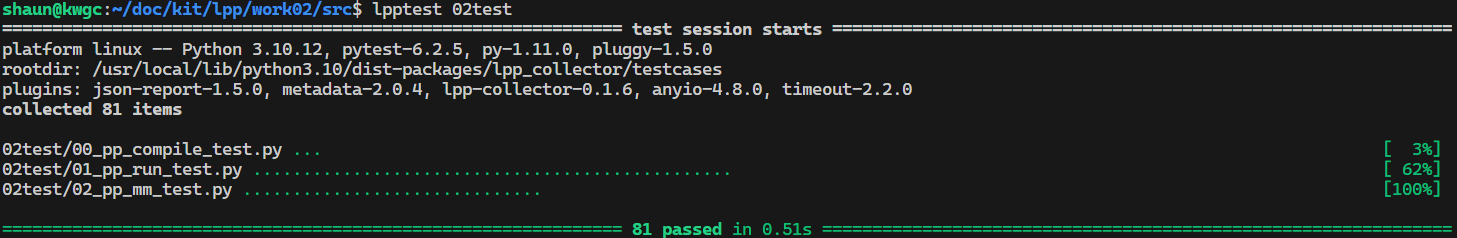
\includegraphics[width=\textwidth]{assets/black_box_test.png}
  \caption{ブラックボックステストの結果}
  \label{fig:black_box_test}
\end{figure}

\subsection{ホワイトボックステスト}
ホワイトボックステストの結果を図\ref{fig:white_box_test}に示す.
\begin{figure}[H]
  \centering
  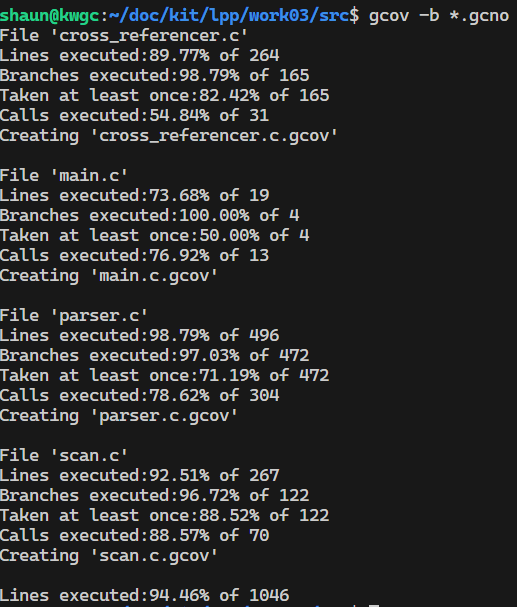
\includegraphics[width=0.6\textwidth]{assets/white_box_test.png}
  \caption{ホワイトボックステストの結果}
  \label{fig:white_box_test}
\end{figure}

\subsection{テストデータの十分性}
ブラックボックステストでは,制約規則のテストが通っているため,少なくとも仕様は満たしていると言える.
ホワイトボックステストについては,図\ref{fig:white_box_test}より今回メインに実装したモジュールを見ると,cross\_referencer.cは命令網羅率が$89.77\%$,条件網羅率が$82.42\%$とやや高水準となっている.
一方,parser.cは命令網羅率が$98.79\%$とかなり高く出たが,条件網羅率が$71.19\%$と相対的に小さくなっている.この2つのモジュールの結果から言えることは,
条件網羅に関してはもう少しテストケースの改善の余地があると言える.だが,決して低い数値ではないため今回は良しとする.

\section{課題のスケジュールと実際の進捗状況}
\subsection{事前計画}
\begin{table}[H]
  \centering
  \caption{課題3の事前計画}
  \begin{tabular}{cccp{10cm}}
    \hline
    開始日 & 終了日 & 予定工数(h) & 作業内容                   \\ \hline
    1/31   & 1/31   & 1           & 資料を読んで仕様をまとめる \\
    1/31   & 1/31   & 2           & 意味解析系の概略設計       \\
    1/31   & 2/2    & 20          & プログラムの作成           \\
    2/1    & 2/3    & 5           & テスト                     \\
    2/3    & 2/3    & 4           & レポートの作成             \\\hline
  \end{tabular}
\end{table}

\subsection{事前課題の立て方についての前課題からの改善点}
前回は資料を読んでからプログラムの作成に移るまでに時間がかかってしまうスケジュールの組み方をしてしまった.
ただでさえ着手が遅いにもかかわらず,読解の工程を作ってしまうとさらに遅くなってしまう.そのため,無理のない範囲で
スケジュールをあえて詰めることで,ある程度の理解度まで達したらプログラム作成に着手できるようにした.

\subsection{実際の進捗状況}
\begin{table}[H]
  \centering
  \caption{課題3の事前計画}
  \begin{tabular}{cccp{10cm}}
    \hline
    開始日 & 終了日 & 工数(h) & 作業内容                   \\ \hline
    1/31   & 1/31   & 2       & 資料を読んで仕様をまとめる \\
    1/31   & 1/31   & 2       & 意味解析系の概略設計       \\
    1/31   & 2/5    & 35      & プログラムの作成           \\
    2/4    & 2/5    & 6       & テスト                     \\
    2/5    & 2/6    & 6       & レポートの作成             \\ \hline
  \end{tabular}
\end{table}

\subsection{当初の事前計画と実際の進捗との差の原因}
1つは,他の課題と並行して行うようなスケジュールを組んだつもりだったが,他の課題を素早く処理できなかったために
本課題の完成にも時間がかかってしまった.そのため,課題に優先順位を付け,本課題を最優先にして進めるべきだった.
また,課題を溜め込んでしまったことが全ての元凶なため,早期の着手を心掛ける必要があった.

プログラムの作成に多くの時間がかかってしまったが,原因は細かいテストを行わずに一気に仕上げようとしてかえって詰まったことにある.
そのため,次回は仕様を少しずつテストしながら進めたい.

\end{document}